\documentclass[a4paper]{report}
\usepackage{fullpage}
\usepackage{alltt}
\usepackage{listings}
\usepackage{caption}
\usepackage{url}
\usepackage{tikz}
\usetikzlibrary{arrows,positioning} 
\tikzset{
    %Define standard arrow tip
    >=stealth',
    %Define style for boxes
    rect/.style={
           rectangle,
           rounded corners,
           draw=black, very thick,
           text width=6.5em,
           minimum height=2em,
           text centered},
    circ/.style={
           circle,
           rounded corners,
           draw=black, very thick,
           text width=6.5em,
           minimum height=2em,
           text centered},
    % Define arrow style
    pil/.style={
           ->,
           thick,
           shorten <=2pt,
           shorten >=2pt,}
}
%\usepackage{courier}

\begin{document}

\lstset{ %
language=Haskell,               % the language of the code
basicstyle=\ttfamily,       % the size of the fonts that are used for the code
numberstyle=\footnotesize,      % the size of the fonts that are used for the line-numbers
stepnumber=2,                   % the step between two line-numbers. If it's 1, each line 
% will be numbered
numbersep=5pt,                  % how far the line-numbers are from the code
showspaces=false,               % show spaces adding particular underscores
showstringspaces=false,         % underline spaces within strings
showtabs=false,                 % show tabs within strings adding particular underscores
tabsize=2,                      % sets default tabsize to 2 spaces
captionpos=b,                   % sets the caption-position to bottom
breaklines=true,                % sets automatic line breaking
xleftmargin=30pt,
breakatwhitespace=false,        % sets if automatic breaks should only happen at whitespace
title=\lstname,                 % show the filename of files included with \lstinputlisting;
escapeinside={\%*}{*)},         % if you want to add a comment within your code
morekeywords={*,...}            % if you want to add more keywords to the set
}


\title{Lazy functional programming language targeting Low Level Virtual Machine}
\author{\textit{Author:}\\Piotr Micha\l{} Kaleta\\\\\emph{Supervisor:}\\dr W\l{}odzimierz Moczurad}
\date{\today}

\maketitle
\pagenumbering{roman}

\newpage
\thispagestyle{empty}
\mbox{}

\Huge
\begin{abstract}
  \normalsize
  \center
  This paper describes the design and Haskell implementation of a lazy
  programming language called Kivi. It is higly influenced on both Haskell's
  syntax as well as the way that computations are performed. However it generates
  the \textit{Low Level Virtual Machine}\cite{website:llvm} Intermediate
  Representation code as the output, which is then assembled and compiled to
  native code by LLVM.
\end{abstract}


\renewcommand{\abstractname}{Acknowledgements}
\begin{abstract}
  \normalsize
  \center
  TODO: napisac
  \begin{flushright}
    Piotr Kaleta
  \end{flushright}
\end{abstract}

\normalsize
\pagenumbering{arabic}

\tableofcontents

\chapter{Introduction}

This paper describes the design and implementation of a lazy functional
language compiler. The implementation is based on the
\textit{G-machine}\cite{jones87} and uses \textit{lazy graph reduction} to
perform evaluation.

The compilation process is implemented as a set of passes that eventually
transforms the source code into simple intermediate language \textit{lambda
calculus} enriched with let(rec) expressions. It would be possible to implement
compiler using less passes than I did, or maybe even one, but such clear
separation made things simpler to both develop and debug as well. Besides now
the compiler is very modular and inserting additional passes could be done with
no harm, which wouldn't be that easy if I'd used one pass only instead.


In following chapters I am going to describe the process of translating
\textit{Lambda Calculus} into \textit{G-code} instructions.  Finally these
instructions will either be evaluated by the interpreter or compiled down to
LLVM intermediate representation and further to native code by LLVM
infrastructure compilers. Design and implementation of both of these concepts
will be described in separate chapters.

TODO: Opis po kolei czesci dokumentu

\section{Implementation language - Haskell}


\chapter{Parsing}

In order to translate the source of \textit{Kivi} into \textit{Lambda Calculus}
it has to be available in a structured form so thate later passes could easily
traverse it. \textit{Abstract Syntax Trees}\cite{wiki:ast} has been widely adopted as a
standard form of keeping the representation of source code in memory. The
process of reading the input source file and producing AST from it is called
\textit{parsing}.
I've chosen to implement a simple parser, in a similar manner as in
\cite{joneslester00} as it seemed as the simplest approach to me then. Now, as
the parser has grown, I'd strongly consider rewriting it to use parser combinator
library such as \cite{website:parsec} instead.  The parsing consists of two
passes. As previously mentioned such separation makes implementation and
reading the code easier. Thus parsing consist of:

\begin{itemize}
  \item Firstly \textit{lexical analysis} implemented by \texttt{lex} in
    \texttt{Lexer.hs} module extracts \textit{tokens} from plain text.
    \textit{Tokenization} is the process of demarcating and possibly
    classifying sections of a string of input characters. The resulting tokens
    are then passed on to further processing.
  \item \textit{Syntax analysis} is the process of analyzing the stream of
    tokens and building an \textit{Abstract Syntax Tree} from it.
\end{itemize}


TODO: Diagram of how parsing process work
TODO: Grammar of the language

This two-phase process is implemented as\footnote{Where \texttt{PatProgram}
is program containing patterns}:

\begin{lstlisting}
parse :: String -> PatProgram
parse = syntax . lex
\end{lstlisting}

\section{Lexical analysis}

The types for lexer are following:
\begin{lstlisting}
type Token = String
type TokenInfo = (Int, Token)
\end{lstlisting}
Where \texttt{TokenInfo} consist of line number and a token string itself.

The heart of \textit{lexical analyser} is the \texttt{lex'} function. It works
by classifying the parts of remaining input based on first characters.
Building number tokens may be a nice example of how it works:

\begin{lstlisting}[label=lst:lex_comment,caption={Building tokens from numbers.}]
lex' (c : cs) lnum | isDigit c =
    (lnum, numToken) : lex' restCs lnum
        where
        numToken = c : takeWhile isDigit cs
        restCs = dropWhile isDigit cs
\end{lstlisting}


\section{Syntax analysis}
\label{sec:syntax_analysis}
Once we can accept tokens from lexer it's time to build a hierarchical
structure called \textit{Abstract Syntax Tree} (or AST for short) from it. ASTs
are tree representations of abstract syntactic structures written in
programming language. Nodes in such tree represent different constructs from
the source code. The word abstract is used because not every detail from source
code has its counterpart in the AST, some unnecessary details are ommited.

Data type for representing Kivi's Abstract Syntax Trees is defined in
\textit{Common.hs} module and it is a parametrized data type. This concept is
a similar idea to templates in C++ or generics in Java. It allows the code to
be reused and forms the basic idea of \textit{parametric poylmorphism}
(see \cite{website:parametric_polymorphism}). The data type definition is
following:
\begin{lstlisting}
data Expr a = EVar Name
            | ENum Int
            | EChar Int
            | EConstrName Name
            | EConstr Int Int
            | EAp (Expr a) (Expr a)
            | ELet IsRec [Defn a] (Expr a)
            | ECase (Expr a) [Alter Pattern a]
            | ECaseSimple (Expr a) [Alter Int a]
            | ECaseConstr (Expr a) [Alter Int a]
            | ELam [a] (Expr a)
            | EError String
            | ESelect Int Int Name
\end{lstlisting}
The \texttt{Expr} data type is parametrized with respect to its binders.
Binders, as name suggests, are used when the variable is being bound to a
value. This happens in lambda abstractions, \texttt{let} and \texttt{letrec}
definitions as well as in \texttt{case} expressions. To give an e example of
how a simple source code construct will look, when parsed to AST,  lets look at
the following example:
\begin{lstlisting}
let
    x = 1;
    y = 2
in
    x + y
\end{lstlisting}
The result returned from \texttt{parse} function will be\footnote{In reality
the output from \texttt{parse} is more complicated because it returns programs
with patterns. However in order to grasp the concept of parametrized
\texttt{Expr} type its easier to forget about that fact for a while.}:
\begin{lstlisting}
  ELet False
       [('x', ENum 1), ('y', ENum 2)]
       EAp (EAp (EVar '+') (EVar 'x')) (EVar 'y')
\end{lstlisting}

Defining expressions in this way greatly reduces the amount of code to be
written. For example, initially parser returns programs with patterns in them,
but later phases of compilation process gets rid of them by transforming
program into a representation that uses \texttt{case} expressions instead.
Thanks to parametrized definition of \texttt{Expr} data type we could define
parse as returning \texttt{Expr Pattern}, whereas later phases return
\texttt{Expr String}.

\section{Implementation of Parser}
TODO: tu mozna napisac jak dziala parser o ile za duzo nie wyjdzie reszty
\subsection{Analysing patterns}
TODO: co tu mialo byc?


\chapter{Translation to Lambda Calculus}

In this chapter I'm going to present the process of transformation of a
high-level functional language into a simple intermediate form - \textit{lambda
calculus}. In the first part I'll show \textit{Kivi}'s syntax, its
constructs and structures. Later on the desired output form -
\textit{Lambda Calculus} will be shown. The rest of the chapter will
consist of ways to translate the first form into another.

\section{Syntax}
Source of \textit{Kivi}'s program consist of set of
\textit{supercombinators}\cite{wiki:supercombinator}. Supercombinator is an
expression consisting of either constants or other supercombinators and
doesn't contain any free variables in its body. Supercombinators might have
arguments, and those which doesn't are called \textit{constant applicative forms}
(or CAFs for short). Listing~\ref{supercombinator_ex} shows the simple
supercombinator with one argument.

\begin{lstlisting}[label=supercombinator_ex,caption={Simple supercombinator.}]
sqr x = x * x
\end{lstlisting}

There is one special supercombinator called \textit{main}, that takes no
arguments. It is the entry point for program execution. If there's no
\textit{main} CAF present in Kivi's source, both compiler and interpreter
should issue specific error message.

\subsection{Case expressions}
The purpose of case expression is to allow the programmer to control the flow
of program execution via a multiway branch. The semantics of case is rather
simple. First, the expression under case is evaluated and then based on result,
the appriopriate execution path is chosen. Example of case expression is
presented in Listing~\ref{lst:case_ex}.

\begin{lstlisting}[label=lst:case_ex,caption={Fibonacci with case}]
fib n =
    case n of
        0 -> 1;
        1 -> 1;
            n -> fib (n-1) + fib (n-2);

main = fib 10
\end{lstlisting}

% TODO: zmienic \ref{xxx} na \ref{lst:xxx}
\subsection{Local bindings}
Supercombinators provides the ability to define local definitions using
\texttt{let} keyword. The scope of variables defined using \texttt{let} is
enclosed by the expression following \texttt{in} keyword. The example use of
local binding is presented in Listing~\ref{let_ex}


\begin{lstlisting}[label=let_ex,caption={Local \texttt{let} binding.}]
sum x y = x + y;

main =
    let x = 1
        y = 2
    in
        sum x y
\end{lstlisting}

\subsection{Recursive local bindings}
In order to define mutually recursive bindings using \texttt{let} one has to use the
special \texttt{letrec} construct as shown in Listing~\ref{factorial_letrec_ex}


\begin{lstlisting}[label=factorial_letrec_ex,caption={Factorial function using \texttt{letrec}.}]
sum x y = x + y;

main =
    letrec fac n =
        case n == 0 of
            True -> 1;
            False -> n * fac (n-1)
    in
        fac 5
\end{lstlisting}

\subsection{Where clauses}
Another way of creating recursive definitions is using the \texttt{where}
clause. Internally it will be translated into letrec binding. Example use of
\texttt{where} clause is shown in Listing~\ref{factorial_where_ex}

\begin{lstlisting}[label=factorial_where_ex,caption={Factorial function using \texttt{where}.}]
main = fac 5
    where
        fac n = case n == 0 of
            True -> 1;
            False -> n * fac (n - 1)
\end{lstlisting}

\subsection{Lambda abstractions}
Functions in Kivi can be defined in two ways. The first one is the top level
supercombinators that has already been discussed. The other option is to define
them as \textit{lambda abstractions}. This concept is similar to \textit{anonymous
functions} used in imperative languages. The syntax for defining lambda
abstractions is presented in Listing~\ref{lambda_ex}.

\begin{lstlisting}[label=lambda_ex,caption={Lambda abstraction}]
f = (\x . x * 2) 42
\end{lstlisting}

In this example the lambda abstraction which doubles the arguments value is
created and then applied to 42 yielding 84 as result.

During compilation process programs containing lambda abstractions are
transformed into their equivalents with lambda abstractions substituted for top
level supercombinators. This process is called \textit{lambda lifting} and is
described in more detail in chapter~\ref{lambda_lifting}.

\subsection{Pattern matching}

Pattern matching consists of specifying patterns to which some data should
conform and then checking to see if it does, as well as deconstructing the data
according to those patterns. So in other words, using pattern matching you can
recognize values, bind variables to those values and break structures down into
parts.
Patterns are matched in order they are defined in source code. Once a
successful branch is found, the right-hand-side expression is evaluated and
result returned. None of the following patterns is checked. If after checking
all patterns it turns out that none of them matches the argument, the error is
returned.

\begin{lstlisting}[label=pattern_matching_ex,caption={Factorial using pattern matching.}]
fac 0 = 1
fac n = n * fac (n - 1)
\end{lstlisting}

In Listing~\ref{pattern_matching_ex} a recursive supercombinator \texttt{fac}
calculating factorial is defined. There are two cases\footnote{To be honest
there are three cases, but for simplicity reasons we assume that
\texttt{fac} is called only for non-negative integers}. Either the
argument is 0 and then the result is 1, or argument is other than than 0 and
then we progress recursively. The factorial definition is expressed very
clearly by means of pattern matching.
Pattern matching is also very useful when it comes to dealing with data
types as we'll see in next section.

\subsection{Structured Data Types}
Data types in Kivi are defined using \texttt{data} keyword, giving the name of
new type as well as its constructors and arities. Together with pattern matching they
provide a very powerful mechanism for dealing with structured entities.

\begin{lstlisting}[label=data_type_ex,caption={Calculating length of list.}]
data List = Nil 0 | Cons 2;

length Nil = 0;
length (Cons x xs) = 1 + length xs
\end{lstlisting}

In Listing~\ref{data_type_ex} a data type \texttt{List} is declared as well as
supercombinator calculating the length of a list by means of pattern matching.
In first case argument is pattern matched to the \texttt{Nil} constructor. If
matching succeeds it means that the list is empty, therefore its length is 0.
In next case the argument is matched to second \texttt{List} constructor, that
is \texttt{Cons}. If argument matches, the \textit{tail} of the list is bound to
\texttt{xs} variable and right hand side of that branch is evaluated.

\subsection{Function application and Currying}
% TODO: write
\section{Lambda Calculus}

\section{Translation to Lambda Calculus}
The process of translating a high-level functional language to \textit{lambda
calculus} might be considered as a set of program transformations. Each such
transformation is meant to simplify \footnote{or help with further
transformations} the program given as its input, eventually leading to the
expected \textit{enriched lambda calculus} form.
All those transformations accept some form of the program as input and yield
the simplified program as output. Therefore we might regard the compilation
process as a function composition of all transformations. This is exactly the
way the compilation is implemented in Kivi, and Haskell lets to express this
in a very concise way:

\begin{lstlisting}
run :: String -> String
run = showResults
    . eval
    . compile
    . lambdaLift
    . lazyLambdaLift
    . analyseDeps
    . transformToLambdaCalculus
    . mergePatterns
    . tag
    . parse
\end{lstlisting}

We have already discussed the parsing in previous chapters, so in the following
sections I'm going to provide a description of all remaining phases.

\section{Structured Data Types and Tagging}
In order to understand the need for this pass one has to know how structured
data types and their constructors are represented internally.
A custom data type declaration in Kivi might look like this one:

\begin{lstlisting}
data Tree = Leaf 1 | Branch 2
\end{lstlisting}

This statement declares the new data type called \texttt{Tree} which can be
constructed in two ways. The common way of looking at the constructors is to
consider them as functions with zero or more arguments that return an instance
of a data type as a result. The \texttt{Tree} constructor is \texttt{Leaf} and
it has no further descendants. It takes one argument which is some kind of
value. The other way to construct a \texttt{Tree} is to create a \texttt{Branch}
taking two children (which also are \texttt{Tree}s) as arguments. For example,
conceptual representation of the following tree is shown in Figure~\ref{fig:tree}:

\begin{lstlisting}
Branch (Leaf 1) (Branch (Leaf 2) (Leaf 3))
\end{lstlisting}

\begin{figure}[h!]
  \centering
    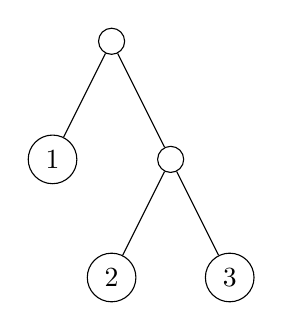
\begin{tikzpicture}
      \tikzstyle{every node}=[circle,draw]
      \node[circle] {}
          child { node[circle] {1} }
          child {
            node[circle] {}
              child { node[circle] {2} }
              child { node[circle] {3} }
          };
    \end{tikzpicture}
  \caption{Example of a tree.}
  \label{fig:tree}
\end{figure}

Constructors are used not only for object creation but also for decomposition
into parts as well as distinguishing the different types of trees based on
constructor. This feature is heavily used when pattern matching. For example
the code in Listing~\ref{lst:sqr_tree} uses it to create a new tree with values
that are square roots of values in original tree.

\begin{lstlisting}[label=lst:sqr_tree,caption={Creating a `square rooted` tree.}]
sqrTree (Leaf v) = Leaf (v * v)
sqrTree (Branch t1 t2) = Branch (sqrTree t1) (sqrTree t2)
\end{lstlisting}

\subsection{Built-in Data Types}
There are few types that are considered built-ins. These are lists, tuples,
and booleans. The ability to think of these common concepts in functional
programming as Structured Data Types makes the implementation straightforward
as I didn't have to treat these entities separately, instead I used a common
notion of data types.
\subsubsection{Booleans}
Boolean values in Kivi are implemented as a regular Structured Data Type having
two constructors representing true and false:

\begin{lstlisting}
data Boolean = True | False
\end{lstlisting}

\subsubsection{Lists}
Lists are structures that allow storing a number of items. They
provide a set of operations on them that allowing to create other
lists\footnote{In Kivi lists as well as other types are immutable, which means
that you cannot modify its contents. Instead you create new values which may
differ from previous ones. }
Kivi provides a variety of way to define a list. First of all lists can be seen
as regular Data Type. Thus there are two constructors for a \texttt{List}
data type. \texttt{Nil} and \texttt{Cons}:

\begin{lstlisting}
data List = Nil 0 | Cons 2
\end{lstlisting}

\texttt{Nil} instantiates an empty \texttt{List} whereas \texttt{Cons} is meant
to \textit{construct} \texttt{List} given two elements: the \textit{head} and
\textit{tail}. List are recursive structures, thus \textit{tail} is another
list.

It turns out that creating a \texttt{List} is a task that occurs very often in
functional languages, therefore it would be nice not to have to write long
constructs such as this one to create 4-element \texttt{List}:

\begin{lstlisting}
Cons 1 (Cons 2 (Cons 3 (Cons 4 Nil)))
\end{lstlisting}

Most functional languages allow programmer to express it in a much shorter way,
and Kivi does it too:

\begin{lstlisting}
[1, 2, 3, 4]
\end{lstlisting}

The same thing concern constructing lists given two elements. Kivi provides
`:`(colon) as construction operator for \texttt{List} type, so the programmer
would write:

\begin{lstlisting}
((2+3) : [1,2,3,4])
\end{lstlisting}
instead of:

\begin{lstlisting}
Cons (2+3)  [1,2,3,4]
\end{lstlisting}

\subsubsection{Tuples}
Tuples are yet another way of storing multiple values in a single one. However
the difference between them and lists is significant. Tuples are
\textit{immutable} in a way that you cannot \textit{cons} to a tuple nor
decompose them into parts using pattern matching. Their main usage is when a
programmer knows in advance how many elements will he need to store.

There is a predefined number of tuple types that you can create, and currently
the bound is set to 4. This means that programmer is not allowed to create
tuples that contain more than 4 elements. This design decision is due to the
fact that from my perspective it's better to use custom Structured Data Type
for readability reasons. The limit of 4 however, is an experimental value and
might be changed.

This all means that tuples with different number of elements are different
types. Therefore there is no such thing as generic `Tuple` type. There are
however \texttt{Tuple0}, \texttt{Tuple1}, \ldots etc., representing tuples with
0 elements, 1 element, \ldots etc.

There are two ways to create a tuple either by using constructors or by a
special \textit{syntactic sugar} construct, similarly as in the case for lists.
These two ways for instantiating a 3-element tuple are equivalent, with the
preference for the second one, due to readability concerns:

\begin{lstlisting}
(((Tuple3 1) 2) 3)
\end{lstlisting}
and
\begin{lstlisting}
(1, 2, 3)
\end{lstlisting}

\subsection{Implementation and tagging}
Internally each data type consist of a list of constructors, each containing a
\textit{tag}, and \textit{arity}. Constructor tags should uniquely identify
each constructor therefore each tag should be different. The definitions
for \texttt{DataType} and \texttt{Constructor} type synonyms, as in
\textit{Common.hs} are as follows:

\begin{lstlisting}
type DataType = (Name, [Constructor])
type Constructor = (Name, Int, Int)
\end{lstlisting}

Because of the fact that there's no way to know in advance how many data type
declarations are there in source file I had to devise some way to assign a
unique tag for each of constructors that is not a built-in one. This is
precisely what the tagging phase is for. It works in two parts:

\begin{itemize}
  \item First it traverses the list of data types and its constructors in order
    to create a mapping between constructor name and its unique tag.
  \item Next the whole AST is recursively traversed and each
    \texttt{EConstrName} node is substituted for \texttt{EConstr} containing
    the previously associated tag and arity.
\end{itemize}

The definitions for those functionalities has been placed in
\textit{AbstractDataTypes.hs} file. This module also contains functionalities
responsible for querying constructors for tags, names, arities as well as
finding constructors given the \texttt{DataType} instance.


\section{Pattern Matching}
This section describes the details and motivation behing pattern matching as
well as describes details of algorithms that transform high-level pattern
matching constructs into enriched lambda calculus.

\begin{lstlisting}[label=lst:length,caption={Calculating length of list.}]
length [] = 0;
length (x : xs) = length xs + 1

length Nil = 0;
length (Cons x xs) = length xs + 1
\end{lstlisting}

Listing~\ref{lst:length} reminds the already well known function for
calculating the length of a list, and also presents the version of the same
function but without \textit{syntactic sugar}. For the purpose of further
discussion lets assume that we're calculating the length of 3-element list:

\begin{lstlisting}
[1, 2, 3]
\end{lstlisting}
which is the same as:
\begin{lstlisting}
Cons 1 (Cons 2 (Cons 3 Nil))
\end{lstlisting}

The way the pattern matching compiler works, is that when length is applied to
an expression it might be not evaluated yet, so in order to proceed we have to
evaluate the function argument. Next, compiler checks whether argument is a Nil
constructor. This is not the case so compiler proceeds to checking against the
second branch. This time it succeeds and \texttt{x} is bound to \texttt{1} and
\texttt{xs} is bound to \texttt{[2, 3]}. The left-hand-sides of function
equations are called \textit{patterns}. They can consist of constructors,
variables, numbers, single characters and strings\footnote{Both the built-in
ones as well as those defined by programmer.}. In previous example we've seen
the combination of those, i.e. The pattern was composed of constructors and
variables. Nothing prevents programmer from creating the so called
\textit{nested patterns}. Example of such situation is present in
Listing~\ref{lst:second_element}, where the function is extracting the second
element from the list.

\begin{lstlisting}[label=lst:second_element,caption={Greatest common divisor.}]
second [] = 0;
second [x] = 0;
second (x1 : (x2 : xs)) = x2
\end{lstlisting}

Patterns in the previous example were not \textit{overlapping}. It
means that changing the order of function equations would not alter the
behaviour of the function. The situation changes when we look at example
presented in Listing~\ref{lst:gcd}.

\begin{lstlisting}[label=lst:gcd,caption={Greatest common divisor.}]
gcd a 0 = a;
gcd a b = gcd b (b % a)
\end{lstlisting}

Here if we've changed the order of equations, the function will never terminate
because the first clause would always match. This kind of patterns are called
\textit{overlapping patterns}.

Pattern matching can occur not only in function equations but also in source
code constructs. It can be used in \texttt{case} expressions as well as in
\texttt{let} and \texttt{letrec} bindings. Examples of those two pattern
matching uses are presented in Listing~\ref{lst:case_pattern_matching} and
~\ref{lst:letrec_pattern_matching}.  Making pattern matching available in
let(rec)s at first sight might look like very similar to other constructs. In
reality, however, it requires quite a complicated additional pass that
transform let(rec)s into more suitable form.  This transformation is described
in more detail in Section~\ref{sec:letrec_transform}.

\begin{lstlisting}[label=lst:case_pattern_matching,caption={Pattern matching in
case expressions.}]
sqrList list =
    case list of
        [] -> []
        (x : xs) -> ((x * x) : sqrList xs)
\end{lstlisting}

\begin{lstlisting}[label=lst:letrec_pattern_matching,caption={Pattern matching
  in let(rec) expressions.}]
let
    (x : xs) = [1, 2, 3, 4];
    (y : ys) = [5, 6, 7, 8]
in
    x + y
\end{lstlisting}

\subsection{Compiling Pattern Matching}
The simplest way to think of pattern matching is to match expression with first
pattern and in case it doesn't match, try the following patterns. Within each
equation patterns are tested from left to right\footnote{In case of functions
with multiple patterns}. Lets consider an example of \texttt{map} function from
Listing~\ref{lst:map}.

\begin{lstlisting}[label=lst:map,caption={Map function example.}]
map f [] = [];
map f (x : xs) = ((f x) : (map f xs));

main = map (\x . x * x) [1, 2, 3, 4, 5]
\end{lstlisting}

The \texttt{map} function returns a list constructed by appling a function
\texttt{f} to all items in a list passed as the second argument. What our
mental model of pattern matching will do when evaluating the \texttt{main}
function, is that it will first try to match the \texttt{(\textbackslash x . x
* x)} lambda abstraction with \texttt{f} variable which will succeed. Matching
any expression to variable will result in success. Then the list \texttt{[1, 2,
3, 4, 5]} will be matched against an empty list - \texttt{[]} and it will fail.
In this situation, according to our simple strategy the algorithm will try to
match the second equation. So it will again try to match the lambda abstraction
with \texttt{f} variable pattern. As we can observe evaluation according to the
simple algorithm might result in redundant computations, and in case of more
complicated patterns it might be a substantial drawback. In order to be able to
perform pattern matching in more optimized fashion we have to transform into
the following form:

\begin{lstlisting}[mathescape=true]
map = $\lambda$ f.$\lambda$ xs.
    case xs of
        Nil       -> Nil
        Cons y ys -> Cons (f y) (map f ys)
\end{lstlisting}

The remaining part of this section contains a description of an algorithm that
is capable of transforming pattern matching into the form that uses case
expressions instead of pattern-matching lambda abstractions, thus allowing to
compile patterns more efficiently. In order to see a more detailed analysis
refer to Chapters 4 and 5 of \cite{jones87}.

\subsection{Pattern-matching Lambda Abstractions}
In lambda calculus, regular lambda abstraction is an expression of the
following form:
\begin{lstlisting}[mathescape=true]
$\lambda x.t$
\end{lstlisting}
where \textit{x} represents a \textit{variable} and \textit{t} stands for
\textit{term}. Intuitively, a lambda abstraction is an anonymous function that
takes a single input, and the \(\lambda\) is said to bind \textit{x} in
\textit{t}, and an application \textit{ts} represents the application of input
\textit{s} to some function \textit{t}. In the lambda calculus, functions are
taken to be first class values, so functions may be used as the inputs to other
functions, and functions may return functions as their outputs.

The difference between regular and pattern-matching lambda abstractions lies in
a fact that instead of variable $x$ on the left side a pattern might be
used. So it might look like that:
\begin{lstlisting}[mathescape=true]
$\lambda p.t$
\end{lstlisting}
where $p$ is a pattern\footnote{Variable is also considered as a
pattern, so regular lambda abstractions form a subset of pattern-matching ones.}

\subsection{Free variables}
\label{sec:free_variable}
A free variable is a notation that specifies places in an expression where
substitution may take place. The idea is related to a placeholder (a symbol
that will later be replaced by some literal string), or a wildcard character
that stands for an unspecified symbol.
In computer programming, a free variable is a variable referred to in a
function that is not a local variable nor an argument of that function:

\subsection{Translating function equations to pattern-matching lambda
abstractions}
For the purpose of further explanations lets consider the following function
definition:

\begin{lstlisting}[mathescape=true]
$f\:p_{1} = e_{1}$
$f\:p_{2} = e_{2}$
   $\vdots$
$f\:p_{n} = e_{n}$
\end{lstlisting}

The pattern matching will be executed from top to bottom until some of them
matches or none of them matches. In the first situation the value of an
expression on the right hand side of matched pattern should be returned and
none of the following patterns should be matched against. In the second one an
error should be reported that no matching branch was found. With this in mind
we can translate the definition of $f$ into following one:

\begin{lstlisting}[mathescape=true]
$f = \lambda x.(((\lambda p_{1}'.e_{1}')\:x)\:[]$
      $((\lambda p_{2}'.e_{2}')\:x)\:[]$
          $\vdots$
      $((\lambda p_{n}'.e_{n}')\:x)\:[]$
      $PatternMatchingError$
\end{lstlisting}
Here, $x$ is a newly introduced variable name to temporarily hold the argument
passed to $f$. The $x$ must not be free in any $e_{n}$ in terms of free
variable definition. Apostrophe means that an expression or pattern has been
translated too. The $[]$ represents an infix function that chooses the next
pattern to match against in case of current pattern's failure.

Lets see our translation in action taking as an example the \texttt{map}
function:
\begin{lstlisting}
map f [] = [];
map f (x : xs) = ((f x) : (map f xs))
\end{lstlisting}
The result of such translation would be following:
\begin{lstlisting}[mathescape=true]
map = $\lambda$f.$\lambda$xs.((($\lambda$Nil.Nil) xs) []
              (($\lambda$(Cons y ys).(Cons (f x) (map f ys))) xs) []
              Error
\end{lstlisting}
In this example $PatternMatchingError$ will never be returned because the set
of constructors $Nil$ and $Cons$ covers the whole domain of constructors for
$List$ data type. It is possible however to construct an example that will cause
that error to occur.

\subsection{Pattern matching algorithm}
\label{sec:pattern_matching_algorithm}

In general a multi-pattern function definition in Kivi of the form:
\begin{lstlisting}[mathescape=true]
$f\:p_{1,1}\:p_{1,2} \dots p_{1,n} = e_{1}$
$f\:p_{2,1}\:p_{2,2} \dots p_{2,n} = e_{2}$
        $\vdots$
$f\:p_{m,1}\:p_{m,2} \dots p_{m,n} = e_{m}$
\end{lstlisting}
is going to be translated into:
\begin{lstlisting}[mathescape=true]
$f = \lambda v_{1}.\lambda v_{2} \dots \lambda v_{n}.((\lambda p_{1,1}'.\lambda.p_{1,2}'\dots\lambda p_{1,n}')\:v_{1}\:v_{2} \dots v_{n})\:[]$
              $((\lambda p_{2,1}'.\lambda.p_{2,2}'\dots\lambda p_{2,n}')\:v_{1}\:v_{2} \dots v_{n})\:[]$
                          $\vdots$
              $((\lambda p_{m,1}'.\lambda.p_{m,2}'\dots\lambda p_{m,n}')\:v_{1}\:v_{2} \dots v_{n})\:[]$
              $PatternMatchingError$
\end{lstlisting}

We've arrived to the point where the pattern matching algorithm starts its
work. The goal is to translate this form into one that uses \texttt{case}
expressions. The code responsible for this task has been placed in
\textit{PatternMatching.hs} module and will be used as a reference. The heart
of algorithm is formed by \texttt{match*} set of mutually recursive functions,
specifically \texttt{matchSc} is the one that performs pattern matching on
supercombinators, and \texttt{matchEquations} matches function definition
equations. \texttt{matchEquations} has the following type signature:

\begin{lstlisting}
matchEquations :: NameSupply
               -> [DataType]
               -> Int
               -> [Name]
               -> [Equation]
               -> Expr Pattern
               -> (NameSupply, Expr Pattern)
matchEquations ns dts n vs eqs def
\end{lstlisting}
where
\begin{itemize}
  \item \texttt{ns}: Name supply for generating new unique names for
    introduced variables. The core logic is implemented in
    \textit{NameSupply.hs} module. It provides a generic facility to generate
    unique names and is used across many modules.
  \item \texttt{dts}: A set of defined data types needed later in constructor
    rule (see ~\ref{sec:constructor_rule}). As shown below \texttt{DataType}
    instances consist of name and list of \texttt{Constructor} instances.
    \texttt{Constructor}s in turn are built from name, tag and arity:

\begin{lstlisting}
type DataType = (Name, [Constructor])
type Constructor = (Name, Int, Int)
\end{lstlisting}

  \item \texttt{n}: The length of the list of argument variables
  \item \texttt{vs}: A list of argument variables. These names are generated
    with the help of \texttt{NameSupply} instance.
  \item \texttt{eqs}: Function equations. They consist of list of patterns as
    well as expression body:
\begin{lstlisting}
type Equation = ([Pattern], Expr Pattern)
\end{lstlisting}
\texttt{Expr Pattern} is a data type for representing expressions that contains
patterns. It uses a parametrized type \texttt{Expr a} where the parameter
\texttt{a} represents type that can be used as function arguments, left-hand
sides of let(rec) bindings, etc. It was previously described in
Section~\ref{sec:syntax_analysis}.
To give an example of how such expression with patterns might look like, let me
show you this \texttt{case} expression:
\begin{lstlisting}
case [1] of
    []       -> 0;
    (x : xs) -> x
\end{lstlisting}
Syntax analyser will transform this source code into the following internal AST
representation\footnote{\texttt{EConstr 2 0} represents a \texttt{Nil}
constructor, whereas \texttt{EConstr 3 2} stands for \texttt{Cons} constructor.}:
\begin{lstlisting}
ECaseConstr ((EConstr 3 2 (ENum 1)) (EConstr 2 0))
            [(PConstr 2 0 [], ENum 0),
             (PConstr 3 2 [PVar x, PVar xs], EVar x)]
\end{lstlisting}

\texttt{Pattern} type instances on the other hand represents patterns itself.
Patterns might be numbers, variables, constructors or special entities standing
for patterns chosen when none of other branches match. Below, the definition of
\texttt{Pattern} type is presented:
\begin{lstlisting}
data Pattern = PNum Int
             | PVar Name
             | PChar Int
             | PConstrName Name [Pattern]
             | PConstr Int Int [Pattern]
             | PDefault
\end{lstlisting}


  \item \texttt{def}: The default expression to evaluate when none of patterns
    matches
\end{itemize}

\texttt{matchEquations} function work according to four rules: the variable,
constructor, mixture and empty ones. The problem of determining which is
applicable given the current state, is solved by looking at first elements of
equations list. Depending on the type of currently considered equation, the
corresponding rule is applied. Helper function \texttt{classifyEquation}
returns the type of equation based on its first element. Following sections
describe each rule in more detail, as well as present a few hopefully
clarifying examples.

Examples in the rest of this section contains a simplified calls to
\texttt{matchEquations} function, where only \texttt{vs}, \texttt{eqs} and
\texttt{def} arguments are presented. The rest of them plays rather a minor
role in understanding the behaviour of algorithm.


\subsection{The Variable Rule}
This rule applies when every equation begins with a variable pattern. In such
case it is possible to remove that variable from every equation and also remove
the corresponding argument variable from \texttt{vs} list. After that we should
transform every expression corresponding to that pattern into one, where every
occurence of removed variable is substituted with the corresponding variable
from \texttt{vs} list. This behaviour is implemented by \texttt{matchVar}
function.
Our previous example, the \texttt{map} function eventually runs into a situation
where variable rule is applicable\footnote{This is a simplified call to
\texttt{matchEquations} where not all arguments are present}:

\begin{lstlisting}[mathescape=true]
matchEquations [$v_{1}$, $v_{2}$]
               [([f, Nil], Nil),
                ([f, Cons y ys], Cons (f y) (map f xs))]
               Error
\end{lstlisting}
After applying the variable rule it would have such form:
\begin{lstlisting}[label=lst:variable_rule, caption={State after applying
  variable rule.}, mathescape=true]
matchEquations [$v_{2}$]
               [([Nil], Nil),
                ([Cons y ys, Cons ($v_{1}$ y) (map $v_{1}$ xs)])]
               Error
\end{lstlisting}

\subsection{The Constructor Rule}
\label{sec:constructor_rule}
Similarly constructor rule is applied when every equation begins with
constructors. Equations are groupped together according to the constructor and
a case expression is introduced in order to choose the right branch. Each group
is now considered separately by recursive calls to \texttt{matchEquation}. New
argument variables are added to each group \texttt{vs} variable according to
the arity of a constructor. This logic has been implemented in
\texttt{matchConstr} function. Again a simple example will clarify this step.

After applying variable rule we've reached the state presented in
Listing~\ref{lst:variable_rule}. Here there are two constructors for two
equations: \texttt{Nil} and \texttt{Cons} so constructor rule applies:

\begin{lstlisting}[label=lst:constructor_rule, caption={State after applying
  constructor rule.}, mathescape=true]
case $v_{2}$ of
    Nil       -> matchEquations []
                                []
                                Error
    Cons $v_{3}$ $v_{4}$ -> matchEquations [$v_{3}$, $v_{4}$]
                                [y, ys]
                                Error
\end{lstlisting}

\subsection{The Mixture Rule}
The need for additional rule arises from the case when neither all equations
begin with variable nor with constructor, hence the name - mixture rule. Here
is an example of function that causes such situation to occur:
\begin{lstlisting}
length (x : xs) = 1 + length xs;
length empty = 0
\end{lstlisting}
After transforming this function we'll get:
\begin{lstlisting}[label=lst:mixture_length, mathescape=true,
  caption={Mixture rule application.}]
matchEquations [$v_{1}$]
               [([Cons x xs], 1 + length xs),
                ([Nil], 0)]
\end{lstlisting}
When such situation occurs, pattern matching algorithm partitions the set of
equations into subsets in a way that each partition contains only elements of
the same type, i.e. In each partition there are only elements that are either
constructors or variables or numbers, etc. This logic is implemented by
\texttt{partition} function in \textit{Utils.hs} module. Once the partitioning
is done it's easy to work out other details. The \texttt{matchEquations} call
from Listing~\ref{lst:mixture_length} is equivalent to following one:
\begin{lstlisting}[mathescape=true]
matchEquations [$v_{1}$]
               [([Cons x xs], 1 + length xs)]
               (matchEquations [$v_{1}$]
                               [([Nil], 0)]
                               Error)
\end{lstlisting}
After evaluating each of the \texttt{matchEquations} calls the length function
will look like this:
\begin{lstlisting}[mathescape=true]
length = $\lambda v_{1}$
    case $v_{1}$ of
        Cons $v_{1}$ $v_{2}$ -> 1 + length $v_{2}$
        Nil       -> 0
\end{lstlisting}


\subsection{The Empty Rule}
Eventually, after applying the previous rules, our algorithm will run into a
situation where the variable list \texttt{vs} is empty, such as the one at
Listing~\ref{lst:constructor_rule} in the case for \texttt{Nil} constructor:
\begin{lstlisting}
matchEquations [] [] expr
\end{lstlisting}
When algorithm arrives into such state, the result is equal to \texttt{expr}.

\subsubsection{Summary}
According to the rules above one can transform every pattern-matching lambda
abstraction to a corresponding (and semantically identical) \texttt{case}
expression. This follows directly from the description of rules.

\section{Transforming \texttt{let(rec)} expressions}
\label{sec:letrec_transform}
The reason why we need to perform \texttt{let(rec)} transformations is due to
the fact that letrec binders\footnote{Binders of a \texttt{let(rec)}
expressions are the left-hand sides of each definition} might contain arbitrary
patterns in them. This prevents us from using the machinery that would be used
instead, if those binders were allowed to be simple variables only. This
section is dedicated to show how the transformation from enriched version of
\texttt{let} and \texttt{letrec} bindings to a simple lambda calculus work in
Kivi. Code implementing functionalities from this section has been placed in
\textit{LetTransformer.hs} module.

The rest of this chapter is devoted to presenting transformations which
translate a program into one, in which only \textit{simple let(rec)}s are
present. Simple \texttt{let(rec)}s are such, that their binders contain only
patterns that are either variable patterns or simple patterns(numbers,
characters, strings, etc.).

The first step of this process is to perform a \textit{conformality
transformation} described in Section~\ref{sec:conformality_transformation}.
Later, general \texttt{let} expressions, are converted into simple
\texttt{let}s via irrefutable \texttt{let}s, obtained by previous
transformation. On the other hand general \texttt{letrec}s are first
transformed into irrefutable \texttt{letrec}s and finally into simple
\texttt{letrec}s. This process is shown in Figure~\ref{fig:letrec_transform}.

TODO: diagram pokazujacy w jakiej kolejnosci sa aplikowane transformacje.

\subsection{Refutable and irrefutable patterns.}
\label{sec:irrefutable_patterns}
We can distinguish two different types of \texttt{let(rec)} bindings:
\textit{Refutable} and \textit{irrefutable} ones. Let's look at this sample
\texttt{let} expression:
\begin{lstlisting}[mathescape=true,label=lst:conformality_check,caption={Pattern matching \texttt{let} binding.}]
let (Cons x xs) = $expr$ in ...
\end{lstlisting}
The problem arises because \texttt{expr} might be evaluated to \texttt{Nil},
and in such situation this pattern matching will fail. This is precisely the
characteristic that distinguishes between the two aforementioned types of
\texttt{let(rec)} bindings. In short refutable bindings are those which contain
at least one refutable pattern and thus may fail during evaluation. On the
other hand irrefutable ones are those in which a failure cannot occur, thus
when all patterns are irrefutable. A pattern is irrefutable if any of these
conditions apply:

\begin{itemize}
  \item It is a simple pattern (i.e. number pattern, character pattern, etc.)
  \item It is a variable pattern
  \item It has the form ($c$ $p_{1}$ $p_{2}$ \ldots $p_{n}$), where $c$ is
    constructor and $p_{1}$ $p_{2}$ \ldots $p_{n}$ are irrefutable patterns
\end{itemize}
The function \texttt{isRefutable} is implemented in exactly this fashion.

\subsection{Conformality transformation}
\label{sec:conformality_transformation}
A \textit{conformality transformation} is an activity to translate the program
into one that checks for patterns mismatch in \texttt{let(rec)} bindings. It
will contain only irrefutable \texttt{let(rec)} bindings. We say that such
program performs a \textit{conformality check}. Lets also mention that such
transformation is only needed in case of refutable bindings, so there's no need
to perform this, possibly expensive, computation in when patterns cannot fail.
So the first step of conformality transformation is partitioning
\texttt{let(rec)} bindings regarding to their refutability. Once we have all
patterns that might fail in one place we need to find a way to transform
\texttt{let(rec)}s into a form that conformality check is done.  Considering
our running example from Listing~\ref{lst:conformality_check} our compiler
would transform this expression into:
\begin{lstlisting}[mathescape=true]
let (Cons x xs) = let $v_{1}$ = $expr$
                  in (($\lambda$p.(Cons x xs)) $v_{1}$) [] Error
\end{lstlisting}
where $v_{1}$ is newly introduced unique variable.

Based on that observation we could derive the general form of conformality
transformation from:
\begin{lstlisting}[mathescape=true]
let $p_{1}$ = $e_{1}$;
    $p_{2}$ = $e_{2}$;
       $\vdots$
    $p_{n}$ = $e_{n}$
in $\ldots$
\end{lstlisting}
into:
\begin{lstlisting}[mathescape=true]
let
    ($c_{k1}$ $v_{1,1}$ $\ldots$ $v_{1,k1}$) = let $w_{1}$ = $e_{1}$
                      in (($\lambda p_{1}$.($c_{k1}$ $v_{1,1}$ $\ldots$ $v_{1,k1}$)) $w_{1}$) [] Error
                               $\vdots$
    ($c_{kn}$ $v_{n,1}$ $\ldots$ $v_{n,kn}$) = let $w_{n}$ = $e_{n}$
                      in (($\lambda p_{n}$.($c_{kn}$ $v_{n,1}$ $\ldots$ $v_{n,kn}$)) $w_{n}$) [] Error
in $\ldots$
\end{lstlisting}
where:
\begin{itemize}
  \item $c_{ki}$ is a constructor of arity equal to the number of variables
    bound by pattern $p_{i}$. Lets call the set of such variables $Var(p_{i})$
  \item $\{v_1, v_2, \ldots, v_n\} = Var(p_i)$
  \item $w_{i}$ is distinct from every $v \in Var(p_i)$
\end{itemize}
The function which calculates the $Var(p_i)$ set is called
\texttt{getPatternVarNames} and its behaviour is works by collecting already
seen variable names while recursively traversing the pattern:

\begin{lstlisting}
getPatternVarNames :: Pattern -> [Name]
getPatternVarNames (PNum n) = []
getPatternVarNames (PChar c) = []
getPatternVarNames (PVar v) = [v]
getPatternVarNames (PConstr tag arity patterns) = foldl collectVars [] patterns
    where
        collectVars vars pattern = vars ++ getPatternVarNames pattern
\end{lstlisting}

The implementation of conformality transformation has been implemented as
\texttt{conformalityTransform} in \textit{LetTransformer.hs}.

\subsection{Transforming irrefutable \texttt{let}s into Simple \texttt{let}s}
As previously mentioned irrefutable \texttt{let} is such that contain only
irrefutable patterns as binders. There are three cases in which we consider a
pattern irrefutable according to definition presented in
Section~\ref{sec:irrefutable_patterns}. In the first two patterns on the
left-had side of definition might be either variable or simple
patterns(numbers, characters, etc.). In such case these patterns are already
simple, so there's nothing else to do. On the other hand when patterns are
irrefutable constructor patterns they are take the following form:
\begin{lstlisting}[mathescape=true]
  let ($c$ $p_1, p_2 \ldots, p_n$) = $expr$ in $\ldots$
\end{lstlisting}
where each $p_1, p_2, \ldots, p_n$ are irrefutable patterns. In order to
convert such expression into a simple \texttt{let}, we can apply the following
transformation\footnote{Without loss of generality we can assume that each
\texttt{let} contains only one definition. Every program could be easily
transformed to conform to this condition.}:
\begin{lstlisting}[mathescape=true]
let $v$ = $expr$
in (let $p_1$ = $Select\mbox{-}r\mbox{-}1$ $v$;
        $p_2$ = $Select\mbox{-}r\mbox{-}2$ $v$;
              $\vdots$
        $p_n$ = $Select\mbox{-}r\mbox{-}n$ $v$
    in $\ldots$)
\end{lstlisting}
Here, $v$ is a newly introduced variable, $r$ is the arity of the $c$
constructor, whereas each $Select\mbox{-}r\mbox{-}i$ is a function that selects
the $i^{th}$ component of a constructor with arity $r$. Again a simple example
should clarify this:
\begin{lstlisting}[mathescape=true]
let (Cons x xs) = (Cons 1 (Cons 2 (Cons 3 Nil)))
\end{lstlisting}
after applying the aforementioned transformation will be converted into:
\begin{lstlisting}[mathescape=true]
let $v$ = (Cons 1 (Cons 2 (Cons 3 Nil)))
in (let x  = $Select\mbox{-}2\mbox{-}1$ $v$;
        xs = $Select\mbox{-}2\mbox{-}2$ $v$)
\end{lstlisting}
$Select\mbox{-}2\mbox{-}1$ when applied to \texttt{(Cons 1 (Cons 2 (Cons 3
Nil)))} will yield \texttt{1}, and $Select\mbox{-}2\mbox{-}2$ is going to return
\texttt{Cons 2 (Cons 3 Nil)}.

\subsection{Transforming irrefutable \texttt{letrec}s into Simple \texttt{letrec}s}
Transformation from irrefutable \texttt{letrec}s into simple ones is almost
identical to that concerning \texttt{let}s except from the fact that variables
from all definitions should be groupped together in order to ensure that
they're visible from other bindings. Here's the general scheme for such
conversion:
\begin{lstlisting}[mathescape=true]
letrec ($c_1$ $p_{1,1}, p_{1,2} \ldots, p_{1,n1}$) = $e_1$
       ($c_2$ $p_{2,1}, p_{2,2} \ldots, p_{2,n2}$) = $e_2$
                $\vdots$
       ($c_k$ $p_{k,1}, p_{k,2} \ldots, p_{k,nk}$) = $e_k$
in $\ldots$
\end{lstlisting}
is going to be translated into following expression:
\begin{lstlisting}[mathescape=true]
letrec
    $v_1$ = $e_1$;
    $p_{1,1}$ = $Select\mbox{-}n1\mbox{-}1$ $v_1$;
              $\vdots$
    $p_{n1,1}$ = $Select\mbox{-}n1\mbox{-}n1$ $v_1$;
    $v_2$ = $e_2$;
    $p_{2,1}$ = $Select\mbox{-}n2\mbox{-}1$ $v_2$;
              $\vdots$
    $p_{n2,1}$ = $Select\mbox{-}n2\mbox{-}n2$ $v_2$;
              $\vdots$
    $v_k$ = $e_k$;
    $p_{k,1}$ = $Select\mbox{-}nk\mbox{-}1$ $v_k$;
              $\vdots$
    $p_{nk,1}$ = $Select\mbox{-}nk\mbox{-}nk$ $v_k$;
in $\ldots$
\end{lstlisting}

\subsection{Summary}
After all these transformations took place, all binders in every
\texttt{let(rec)} expressions should become variable pattern in form
\texttt{PVar v = $expr$} or simple pattern. Now the pattern-matching algorithm,
described in Section~\ref{sec:pattern_matching_algorithm} can be used because
it was developed under assumption that left-hand sides of \texttt{let(rec)}
binders doesn't contain refutable and complex patterns. Therefore it is
important to run the conformality transform before pattern matching phase.

\section{Transforming \texttt{case} expressions}
\section{Dependency Analysis}
\section{Lambda Lifting}
\section{Lazy Lambda Lifting}
\section{Type Checker}


\chapter{G-Machine}
\section{Interpreter}
\section{LLVM Compiler}

\bibliographystyle{alpha}
\bibliography{kivi}

\end{document}
